%\chapter*{附錄：大災難多久？但以理書的七十個七}
%\phantomsection
%\addcontentsline{toc}{chapter}{附錄：大災難多久？但以理書的七十個七}
%\markboth{附錄：大災難多久？但以理書的七十個七}{附錄：大災難多久？但以理書的七十個七}

%\setcounter{figure}{0}
%\renewcommand{\thefigure}{\arabic{figure}}   % this is the line that fixes \ref
%\def\theHfigure{appendix.\arabic{figure}}




%\appendix
\renewcommand{\appendixname}{附錄}
\renewcommand{\thechapter}{\arabic{chapter}}
\renewcommand{\thefigure}{\appendixname~\thechapter.\arabic{figure}}  % Appendix 1.1, 1.2, …

\refstepcounter{chapter}
\chapter*{附錄：大災難多久？但以理書的七十個七}
\addcontentsline{toc}{chapter}%
  {\appendixname~\thechapter\quad 大災難多久？但以理書的七十個七}





\section*{一般說法：「七年」的大災難}
以下是前千禧年派的觀點。
但以理書9章是理解末後年日的關鍵。
\begin{ScriptureBox}

\item[9:24] 為你本國之民、和你聖城、已經定了七十個七、要止住罪過、除淨罪惡、贖盡罪孽、引進〔或作彰顯〕永義、封住異象和預言、並膏至聖者。〔者或作所〕
\item[9:25] 你當知道、當明白、從出令重新建造耶路撒冷、直到有受膏君的時候、必有七個七、和六十二個七．正在艱難的時候、耶路撒冷城連街帶濠、都必重新建造。
\item[9:26] 過了六十二個七、那受膏者〔那或作有〕必被剪除、一無所有、必有一王的民來毀滅這城、和聖所．至終必如洪水沖沒、必有爭戰．一直到底、荒涼的事已經定了。
\item[9:27] 一七之內、他必與許多人堅定盟約、一七之半、他必使祭祀與供獻止息．那行毀壞可憎的〔或作使地荒涼的〕如飛而來、並且有忿怒傾在那行毀壞的身上、〔或作傾在那荒涼之地〕直到所定的結局。

\end{ScriptureBox}

天使對但以理說，神為以色列民和耶路撒冷「已經定了七十個七」。
這裡的「七」原文是「七的單位」，按上下文指的是「年」，所以70個七就是 $70 \times 7 = 490$ 年。
第70個七，是大災難時期，是七年。

以上的「7個七」（49年）和「62個七」（434年），在歷史上已經應驗。
\begin{itemize}
\item 「7個七」（49年）：一般認為這是指波斯王亞達薛西在位第二十年（約主前445年）給尼希米的命令（尼希米2:1-8）。是從「重新建造耶路撒冷」開始。
\item 「62個七」（434年）：與前一段合計69個七，也就是483年。如果按聖經預言中常用的一年360日計算，483年約為173,880日，正好落在主耶穌騎驢進耶路撒冷、被尊為君王的時候。「那受膏者必被剪除，一無所有」，明確指向基督被釘十字架。\footnote{之後「必有一王的民來毀滅這城和聖所」，這在主後70年羅馬軍隊攻陷耶路撒冷、焚毀聖殿時應驗了。}
\end{itemize}

\section*{大災難是第70個七}

讀者已經發現，「70的七」不是連續的。過去的69個七，已經發生了，而「第七十的七」是未來式。中間有一個很大的空檔。

一個比較廣為接受的解釋，是如圖所示的時間軸。從遠處看一座山脈，前後兩座山峰好像緊緊相連，走近了才發現中間隔著深谷。舊約先知看將來的事也是如此。他們看見了「山峰」：彌賽亞受苦、彌賽亞得榮耀、末日的審判。這些事在他們眼中並列在一起，但他們沒有看見其間那段時間的「山谷」，也就是今天的教會時代。這是所謂的「預言的透視」（prophetic perspective），中文有時簡稱為「山峰觀」\footnote{也叫「預言的望遠鏡效應」（prophetic telescoping）或「預言的透視縮短」（prophetic foreshortening）。}

{
\begin{figure}[htbp]
    \centering
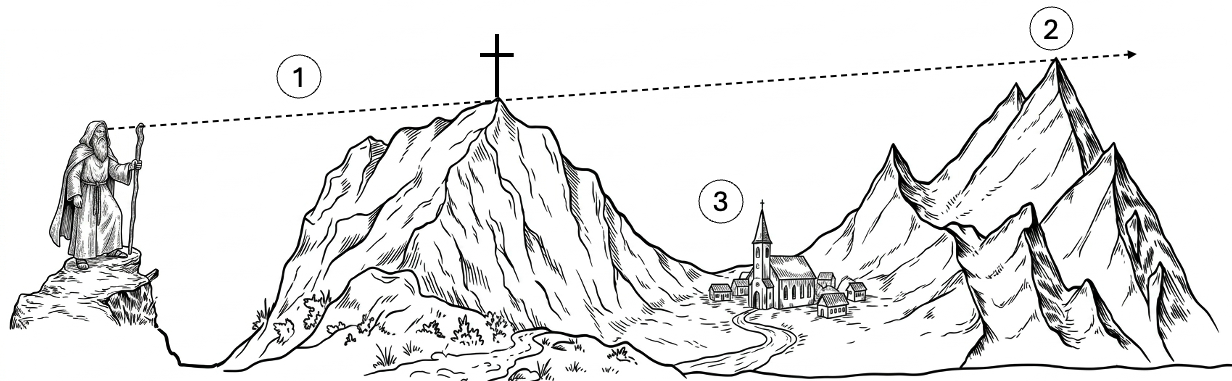
\includegraphics[
    width=1\textwidth, 
    trim=0 0 0 0, 
    clip]{images/mountain_peak_valley.png}
    \caption{「山峰觀」看「七十個七」}
    \label{fig:valley}
\end{figure}
}

\normalsize

圖 \ref{fig:valley}的
\ding{172}的期間是已經應驗的483年。\ding{173}是最後一個七，是先知所見的大災難七年。\ding{174}是山谷，是舊約先知們未見的奧秘，也就是教會的恩典時期。


為什麼山谷被隱藏？保羅說，教會是「奧秘」，「這奧秘在以前的世代、沒有叫人知道、像如今藉著聖靈啟示他的聖使徒和先知一樣．」（以弗所書3:5） 以及「這道理就是歷世歷代所隱藏的奧秘、但如今向他的聖徒顯明了．」（歌羅西書1:26）\footnote{更清楚的例子，是主耶穌在拿撒勒會堂讀以賽亞書61章，讀到「報告神悅納人的禧年」就停下來，把書捲起，說：「今天這經應驗在你們耳中了。」祂沒有讀下一句「和我們神報仇的日子」。在以賽亞書裡，這兩句只隔著一個逗號。在歷史上，卻已經相隔至少兩千年。（以賽亞書61:1-2與路加福音4:18-21）。因此，70個七中間有間隔的讀法並不是解經家憑空加上去的，而是與整本聖經預言一貫的寫法一致。}\footnote{並不是所有解經家都認為第69個七和第70個七之間有間隔。有些人（多屬無千禧年派或過去派）主張70個七是一段不間斷的490年。不過解經上時間對不上。造成更大的問題。在此因為已經超出本書範圍，不再贅述。}


\section*{七年的大災難：前三年半、後三年半}
經文還特別指出：「一七之半，他必使祭祀與供獻止息」，並設立「那行毀壞可憎的」。主耶穌在橄欖山講論中直接引用了這句話：「你們看見先知但以理所說的那行毀壞可憎的站在聖地……那時必有大災難」（馬太福音24:15、21）。由此可見，大災難總共七年，並以中間點為分水嶺。前三年半，敵基督假裝和平，與以色列立約。後三年半，他撕毀盟約，褻瀆聖殿，災難急劇加重，這就是狹義的「大災難」。

這三年半在聖經中有多種一致的說法：「一載二載半載」（ 1 + 2 + $\frac{1}{2}$ = 3 $\frac{1}{2}$）、「四十二個月」、「一千二百六十天」。這些經文互相印證，可見但以理所說的「一七」和「一七之半」都是確切的年日，不只是象徵。所以，大災難多久？按但以理書9章的框架，是七年，其中最嚴厲的「大災難」是後半段的三年半。